\section{Conclusion}
\label{sec:conclusion}

First it can be stated, that already simple tests (such as CenterPixel) lead to reasonable results. But to improve the result significantly, more complicated tests are necessary. Figure~\ref{fig:learner_dist} shows the distribution of chosen weak learners during an average training. The most important weak learner is still CenterPixel
followed by two other very simple learners: GradientNode, TwoPixelNode. The more sophisticated learners HaarWavelet and SURFFilter are chosen rarely.

\begin{figure}
	\centering
	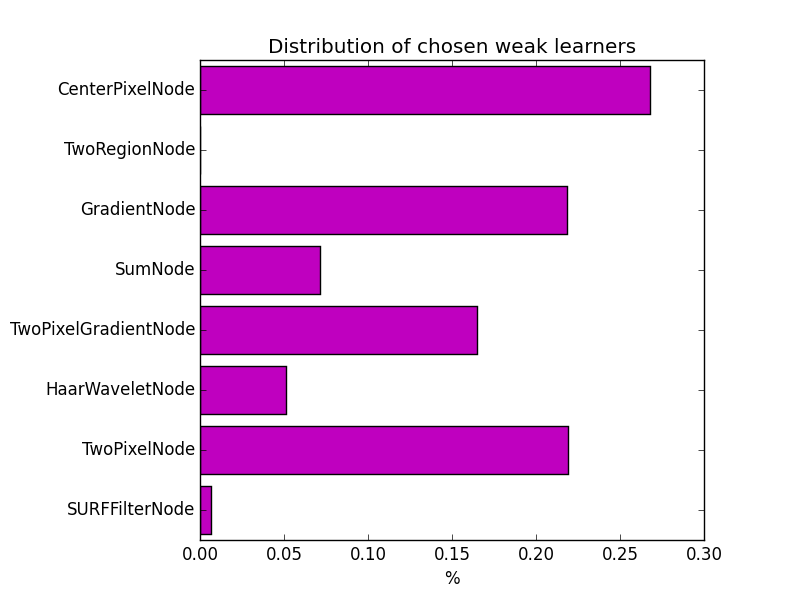
\includegraphics[width=0.8\textwidth]{plots/weak_learner_distribution.png}
	\caption{Distribution of weak learners chosen during training.}
	\label{fig:learner_dist}
\end{figure}

By comparing Figure~\ref{subfig:result_heatmap_xacc_100} with Figure~\ref{subfig:result_heatmap_xacc_150} it seems that the number of trees is not taking any notable effect on accuracy. But by taking into account Figure~\ref{subfig:result_heatmap_iacc_100} and Figure~\ref{subfig:result_heatmap_iacc_150} it shows that the number of trees has an effect. Nevertheless, it also shows that tree depth is the majority to boost performance in accuracy sense. In terms of time performance, tree depth is also a majority because the needed time for training increases exponential by depth. This results also from the fact that the training of trees can easily be parallelized whereas the single node can not. Also a crucial parameter is the number of feature tests per node, which increase training time by a linear factor. But while the training phase time depends highly on the parameters the consumed time during testing is not changing significantly.

